% Fig. 3 -- Simulated active-learning protocol used to evaluate the loop
% without user effort: a ground-truth oracle stands in for the user.
\documentclass[tikz,border=2pt]{standalone}
\usepackage[T1]{fontenc}
\usepackage[scaled=0.92]{helvet}
\renewcommand{\familydefault}{\sfdefault}
\usetikzlibrary{arrows.meta,positioning,fit,backgrounds,calc}

\begin{document}
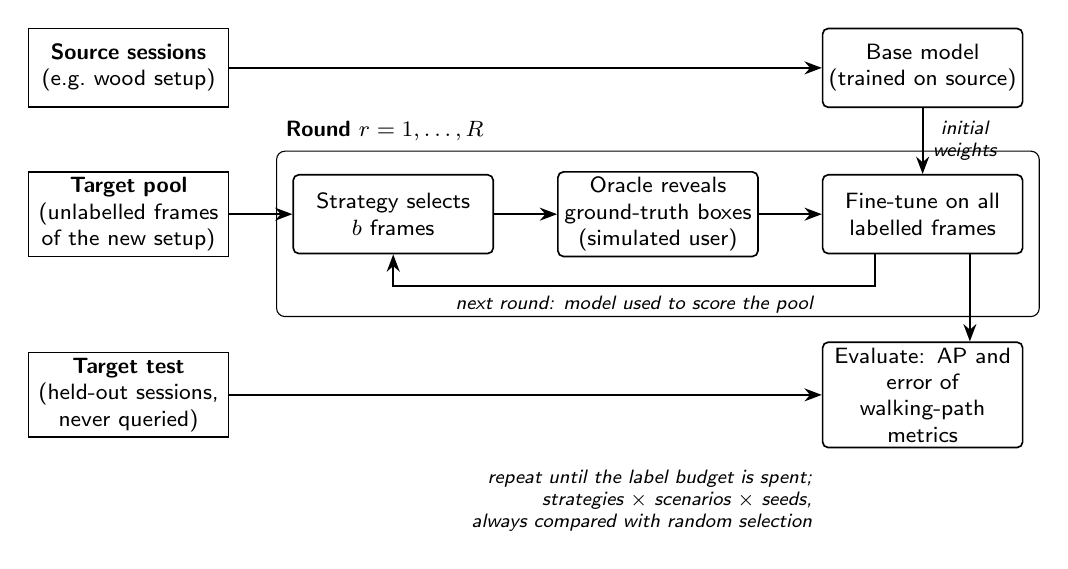
\begin{tikzpicture}[
  font=\footnotesize,
  >={Stealth[length=2.2mm]},
  box/.style={draw, rounded corners=2pt, align=center, minimum height=10mm,
              text width=24mm, inner sep=2pt, line width=0.6pt, fill=white},
  set/.style={draw, align=center, minimum height=10mm, text width=24mm,
              inner sep=2pt, line width=0.6pt},
  flow/.style={->, line width=0.7pt},
  lbl/.style={font=\scriptsize\itshape, align=center},
]
% columns: data | select | oracle | fine-tune
\node[set] (src) {\textbf{Source sessions}\\(e.g.\ wood setup)};
\node[set, below=8mm of src] (pool) {\textbf{Target pool}\\(unlabelled frames\\of the new setup)};
\node[set, below=12mm of pool] (test) {\textbf{Target test}\\(held-out sessions,\\never queried)};

\node[box, right=8mm of pool] (sel) {Strategy selects\\$b$ frames};
\node[box, right=8mm of sel] (oracle) {Oracle reveals\\ground-truth boxes\\(simulated user)};
\node[box, right=8mm of oracle] (ft) {Fine-tune on all\\labelled frames};
\node[box] (base) at (ft |- src) {Base model\\(trained on source)};
\node[box] (eval) at (ft |- test) {Evaluate: AP and\\error of walking-path\\metrics};

\draw[flow] (src) -- (base);
\draw[flow] (base) -- node[lbl, right] {initial\\weights} (ft);
\draw[flow] (pool) -- (sel);
\draw[flow] (sel) -- (oracle);
\draw[flow] (oracle) -- (ft);
\draw[flow] (ft.south) ++(-6mm,0) -- ++(0,-4mm) -| node[lbl, pos=0.25, below] {next round: model used to score the pool} (sel.south);
\draw[flow] (ft.south) ++(6mm,0) -- ([xshift=6mm]eval.north);
\draw[flow] (test) -- (eval);

\begin{scope}[on background layer]
\node[draw, line width=0.4pt, rounded corners=3pt, inner sep=2mm, fit=(sel)(oracle)(ft),
      yshift=-2.5mm, minimum height=21mm,
      label={[font=\footnotesize\bfseries, anchor=south west]north west:Round $r = 1,\dots,R$}] {};
\end{scope}

\node[lbl, below=1.5mm of eval.south west, anchor=north east, text width=70mm, align=right]
  {repeat until the label budget is spent; strategies $\times$ scenarios $\times$ seeds,\\always compared with random selection};
\end{tikzpicture}
\end{document}
